\documentclass[10pt,t,handout]{beamer}
\usepackage{graphicx}
\usepackage{color}
\definecolor{myblue}{rgb}{.8, .8, 1}
\usepackage{amsmath}
\usepackage{empheq}
\usepackage[skins,theorems]{tcolorbox}
\tcbset{highlight math style={enhanced,
  colframe=red,colback=white,arc=0pt,boxrule=1pt}}




\usetheme{Copenhagen}
\title{Scalar radiation from symmetron field oscillations}
\subtitle{\small PIC1 Scientific project}
\author{\textbf{Sebastião Fonseca}}
\institute{Under the supervision of Javier Rubio \\ \,  \\ Departamento de Física \\Instituto Superior Técnico - ULisboa}
\date{27/06/2022}
\titlegraphic{
\includegraphics[width=0.4\textwidth]{Images/ist.png}}
\begin{document}

\frame{\titlepage}

\begin{frame}
\frametitle{Introduction}
\begin{itemize}[<+->]
    \item \small In the standard model of cosmology, ($\Lambda$CDM), the acceleration of the universe is explained by a cosmological constant $\Lambda$
    \item \small Modified theories of gravity have emerged as an alternative by introducing a new scalar field mediating a fifth force, altering the behaviour of gravity
    \item \small General relativity has been tested with high precision, placing constraints on this new force
   
\end{itemize}
\centering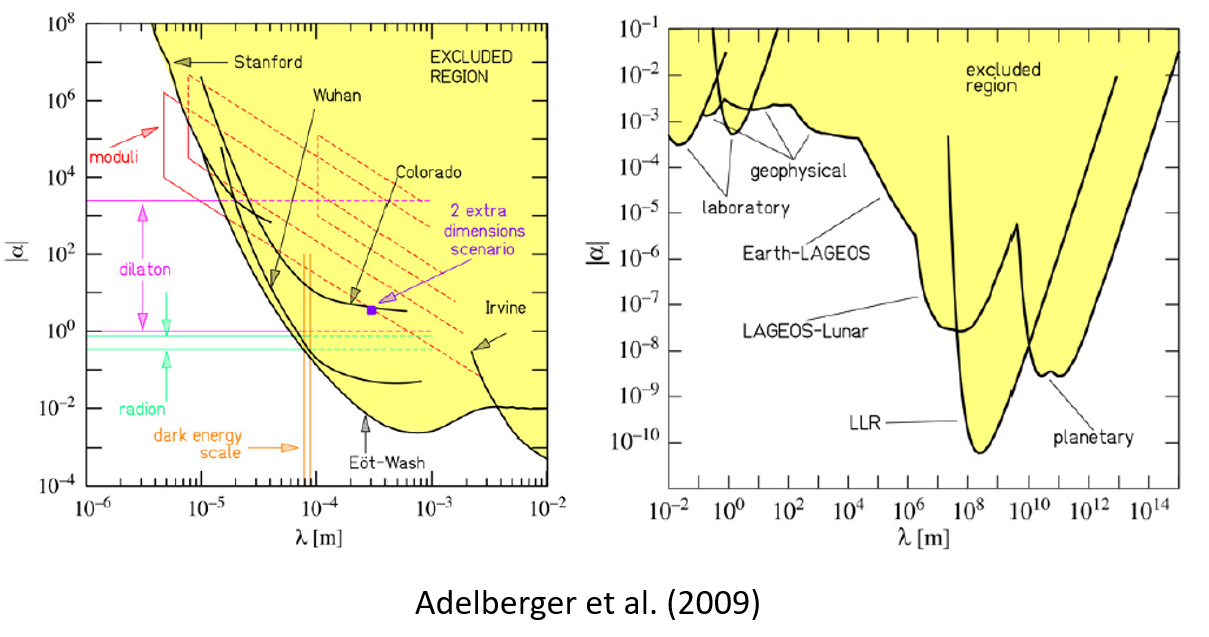
\includegraphics[width=0.8\textwidth]{Images/Constraints.png}
     
\end{frame}
\begin{frame}
\frametitle{Screening mechanisms and scalar waves}
\begin{itemize}[<+->]
    \item \small Screening mechanisms suppress the field in regions of high matter density, hiding fifth forces from local gravity tests
    \item \small Due to the coupling of these fields to mass density, radially pulsating astrophysical objects can source scalar waves.
    \item \small These waves would cause deviations from General Relativity which could be tested by gravitational wave detectors 
    %\item \small In this project this possibility was studied for the symmetron screening mechanism
    
\end{itemize}
\centering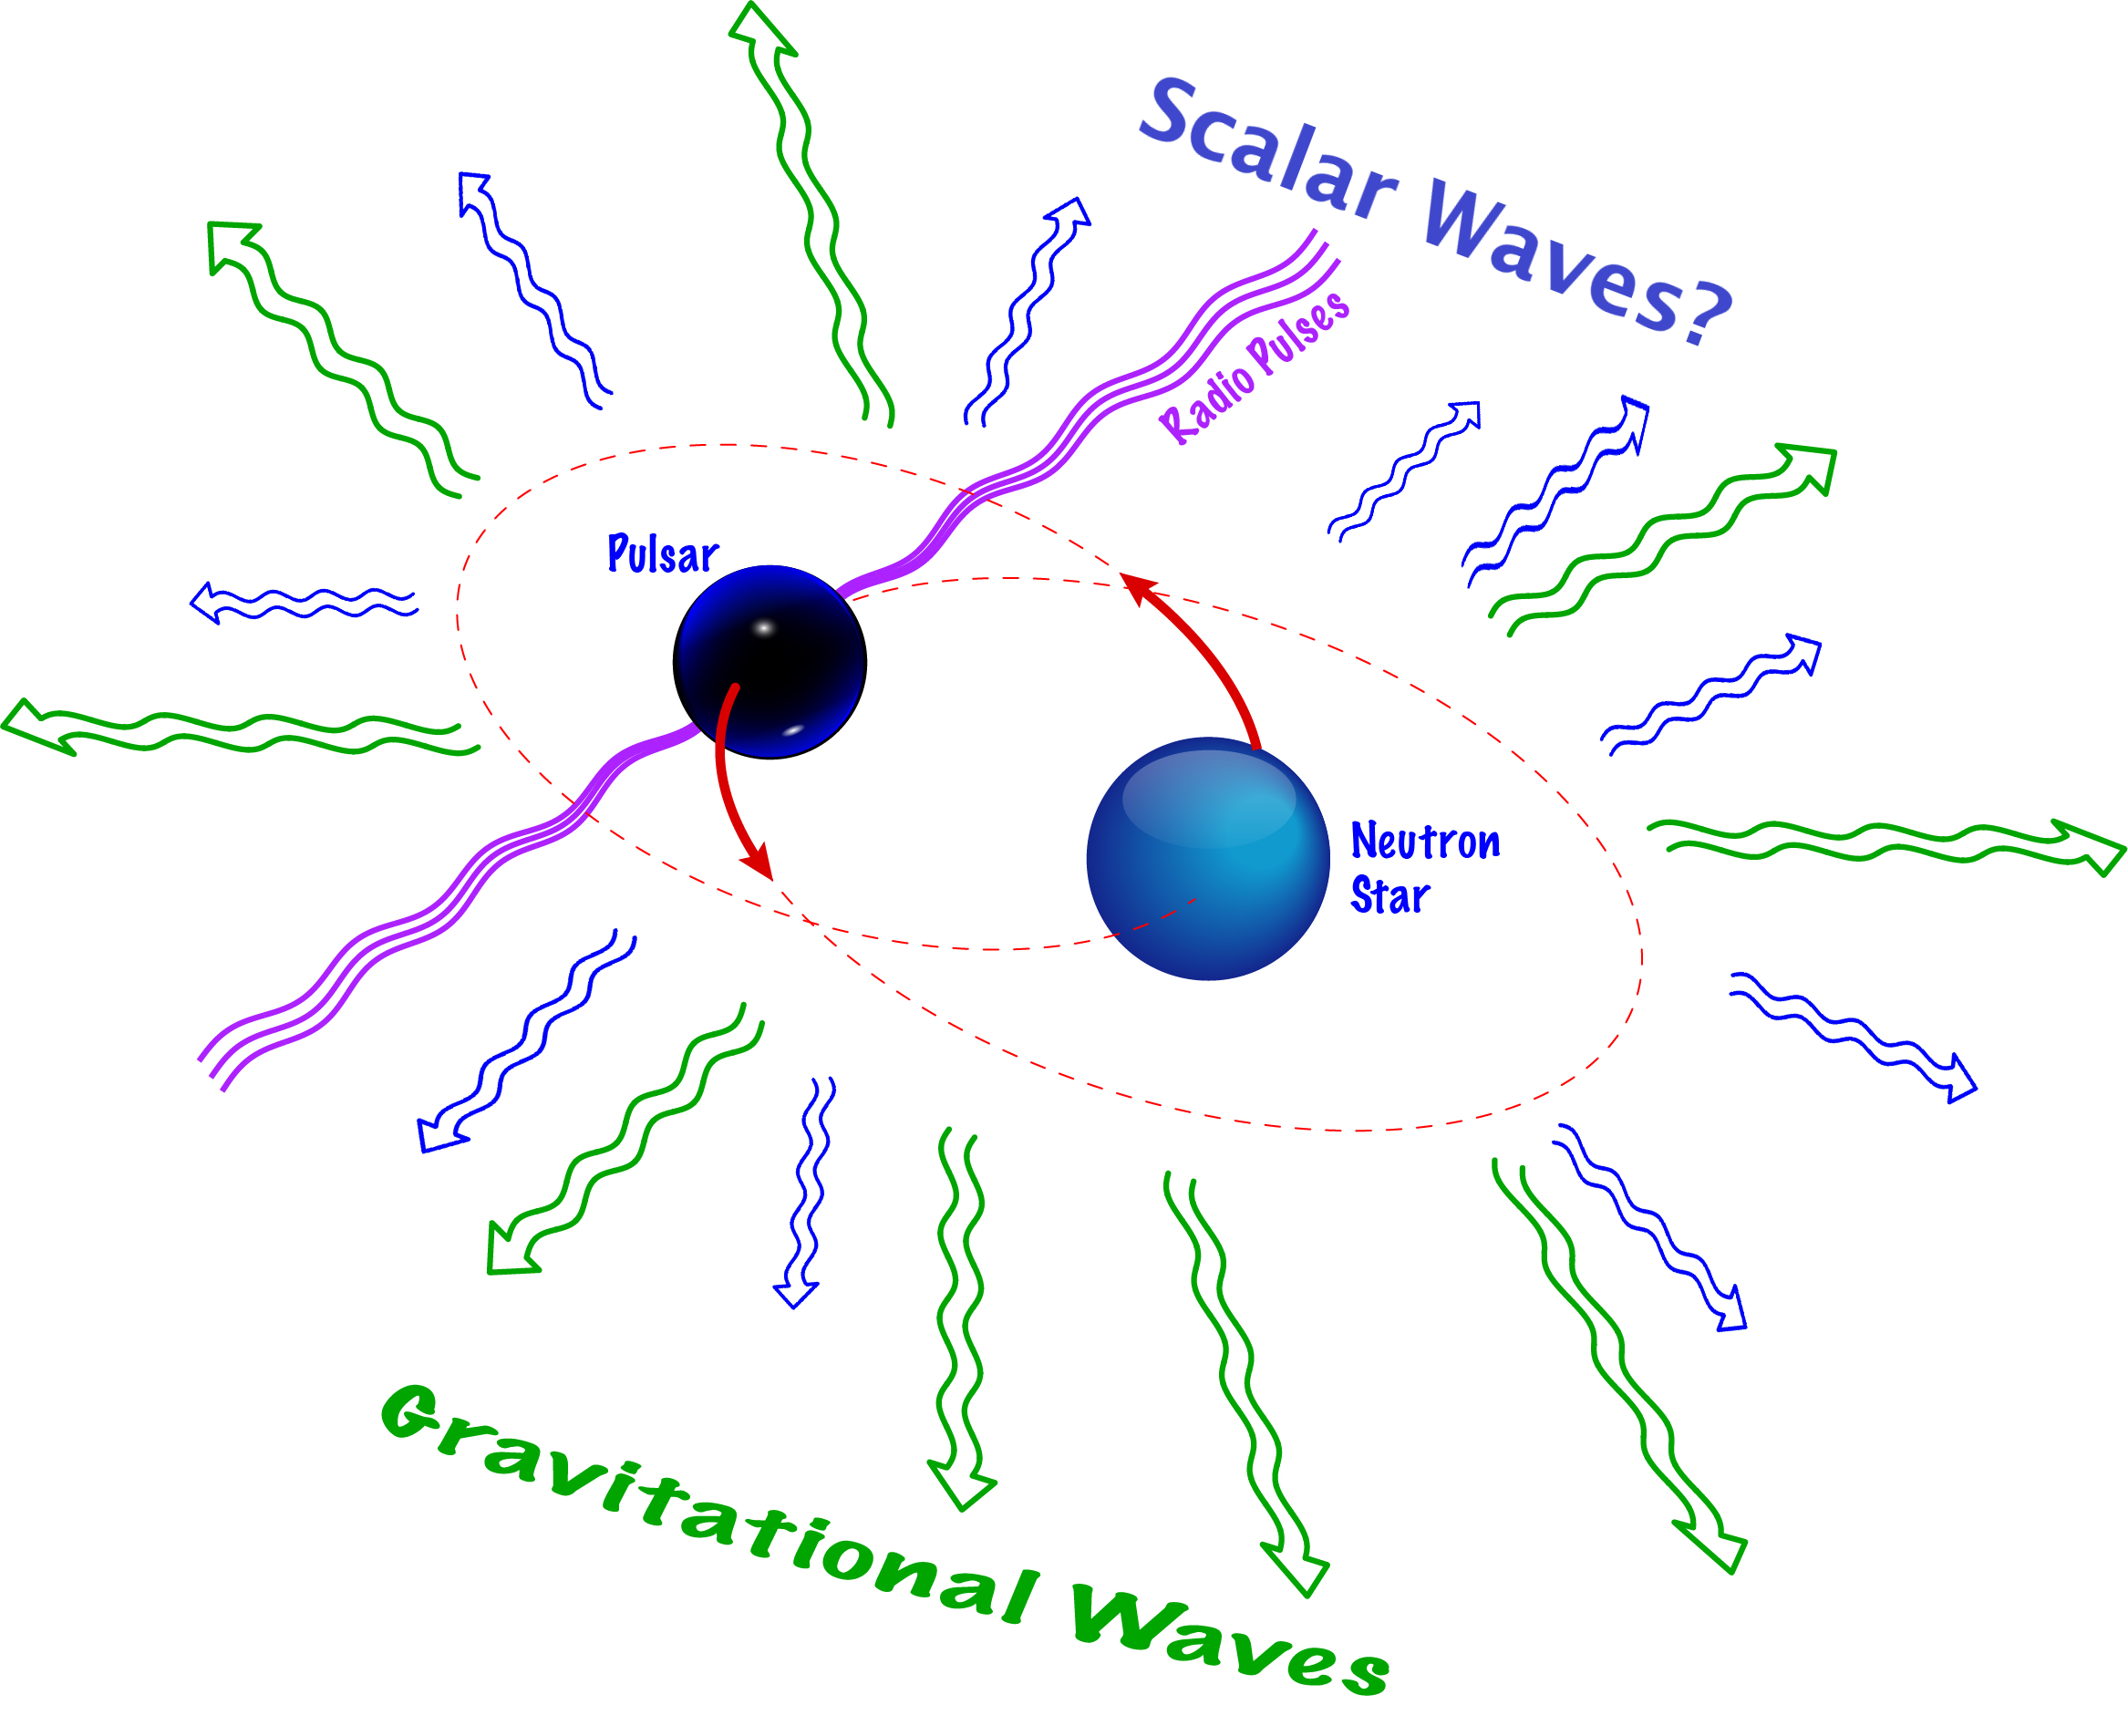
\includegraphics[width=0.6\textwidth]{Images/Final.png}
     
\end{frame}

\begin{frame}{The symmetron}
    \small The symmetron screening mechanism works by combining a symmetry breaking potential with a coupling to the local matter density

    \begin{equation*}
    \tcbhighmath[boxrule=2pt,arc=1pt,colback=blue!10!white,colframe=blue]{ \small V_{\rm eff}(\phi) = \frac{1}{2}\left(\frac{\rho}{M_s^2}-\mu^2 \right)\phi^2 +\frac{1}{4}\lambda\phi^4 }
    \end{equation*}
    %\centering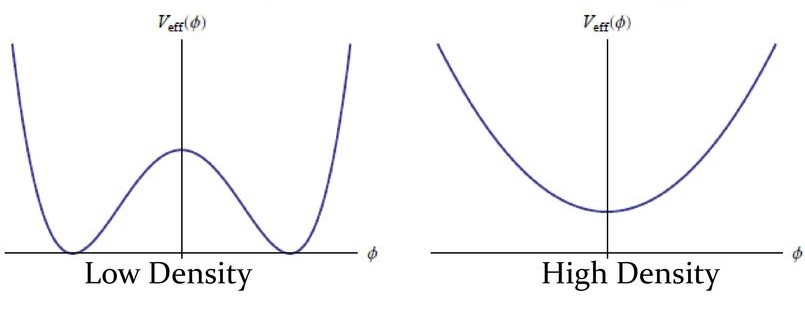
\includegraphics[width=0.65\textwidth]{Images/symmetry.jpg}
    \begin{columns}[T]
    \begin{column}{0.5\textwidth}
    \centering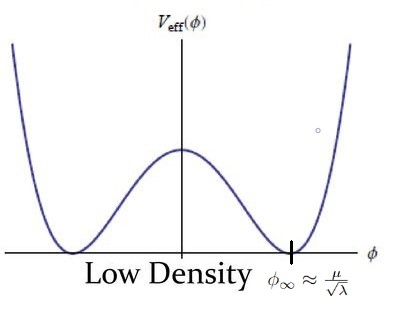
\includegraphics[width=0.55\textwidth]{Images/2.jpg}
    \begin{equation*}
       \small \rho \ll \mu^2M_s^2
    \end{equation*}%\vspace{1mm}
    \begin{equation*}
        \tcbhighmath[boxrule=2pt,arc=1pt,colback=white,colframe=blue]{\small \phi_{\infty} \approx \mu/\sqrt{\lambda}}\hspace{1cm}m_{\infty} \approx \sqrt{2}\mu
    \end{equation*}
    \end{column}
    
    \begin{column}{0.5\textwidth}
    \centering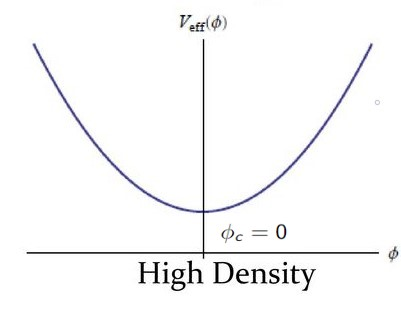
\includegraphics[width=0.55\textwidth]{Images/1.jpg}
    \begin{equation*}
       \small \rho \gg \mu^2M_s^2
    \end{equation*}%\vspace{1mm}
    \begin{equation*}
       \tcbhighmath[boxrule=2pt,arc=1pt,colback=white,colframe=blue]{\small \phi_{c} = 0} \hspace{1cm} m_c = \sqrt{\frac{\rho}{M_s^2}-\mu^2}
    \end{equation*}
    
    \end{column}
    \end{columns}
    
\end{frame}

\begin{frame}
\frametitle{The model}
    Approximations:
\begin{enumerate}
    \item  Newtonian limit
    \item  Constant density and radius
    \item  Radial pulsations with constant amplitude and  frequency 
    \item  The surrounding region is a perfect vacuum 
    
\end{enumerate}
\vspace{5mm}
\centering 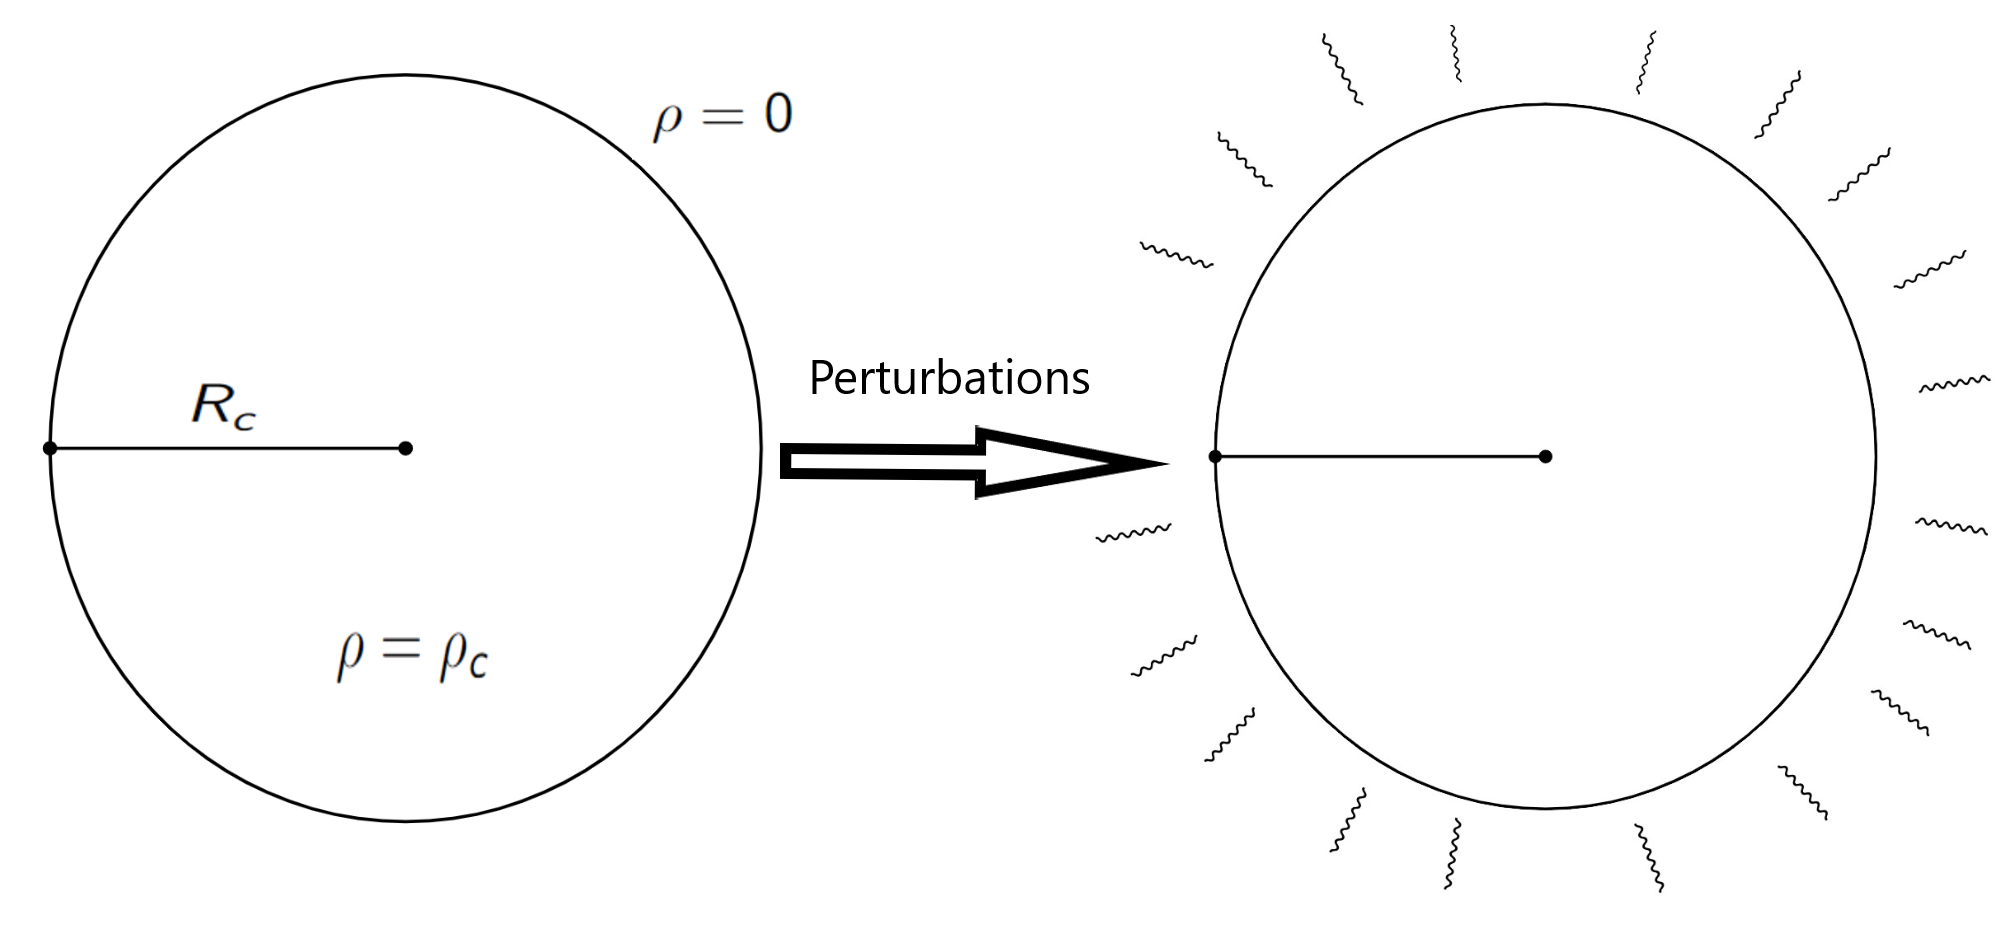
\includegraphics[width=9cm]{Images/YE.png}
\end{frame}

\begin{frame}
\frametitle{Static profile}
    \centering Static equation of motion in spherical coordinates
    \begin{equation*}
        \tcbhighmath[boxrule=2pt,arc=1pt,colback=blue!10!white,colframe=blue]{\frac{d^2\phi_0}{dr^2} + \frac{2}{r}\frac{d\phi_0}{dr} = \left(\frac{\rho_0}{M_s^2}-\mu^2 \right)\phi_0 +\lambda\phi_0^3}
    \end{equation*}
    
    \begin{columns}[T]
    \begin{column}{0.7\textwidth}
    \vspace{.7cm}
    \centering 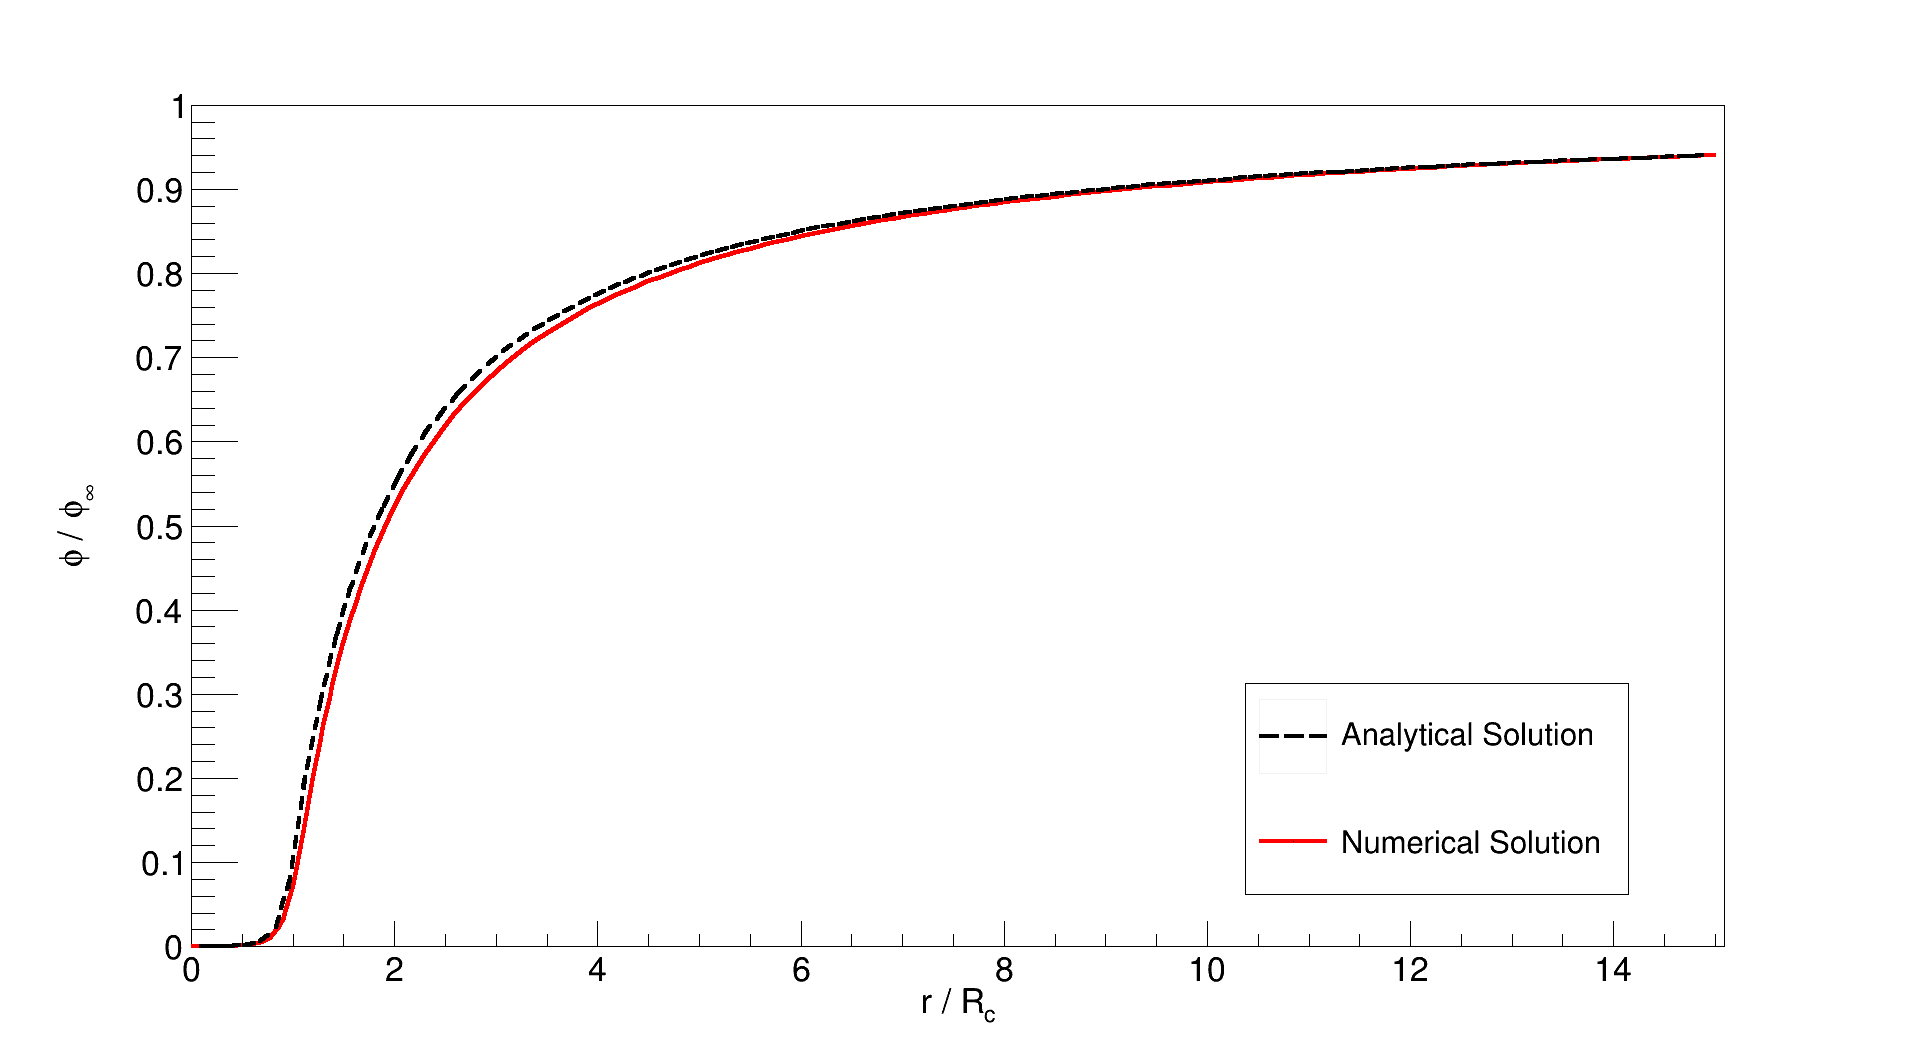
\includegraphics[width=7cm]{Images/Static.png}
    \end{column}
    
    \begin{column}{0.3\textwidth}
    \centering 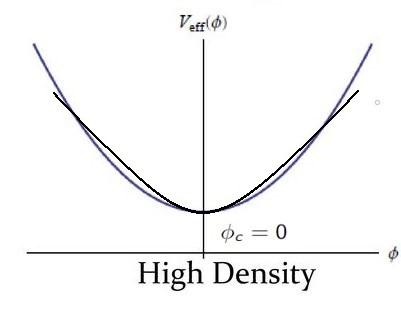
\includegraphics[width=3.5cm]{Images/11.jpg}
    \centering 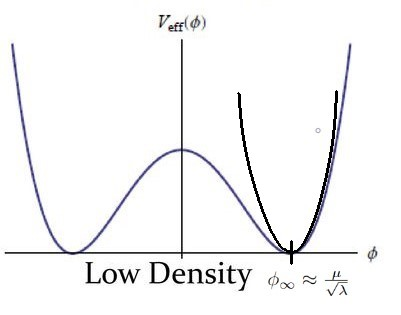
\includegraphics[width=3.5cm]{Images/22.jpg}
    \end{column}
    \end{columns}

    
\end{frame}

\begin{frame}
\frametitle{Perturbations profile}
   \centering Introducing the perturbations into the system

    \begin{equation*}
        \phi(r,t) = \phi_0(r) + \delta\phi(r,t) \hspace{2cm} R(t) = R_c + \Delta R sin(\omega t)
    \end{equation*}
    
    \begin{equation*}
       \implies \tcbhighmath[boxrule=2pt,arc=1pt,colback=white,colframe=blue]{\rho(r,t) = \rho_0(r)\left(1 + 3\frac{\Delta R}{R_c} \sin(\omega t)\right)}
    \end{equation*}
    
    \begin{equation*}
        x \equiv \frac{r}{R_c}\, \hspace{10mm}    \tau \equiv \frac{t}{R_c}\, \hspace{10mm} \varphi \equiv \frac{\phi}{\phi_{\infty}}
    \end{equation*}
    
    
    
    \begin{equation*}
       \small \tcbhighmath[boxrule=2pt,arc=1pt,colback=blue!10!white,colframe=blue]{-\frac{\partial^2\delta\varphi}{\partial\tau^2}+\frac{\partial^2\delta\varphi}{\partial x^2}+\frac{2}{x}\frac{\partial\delta\varphi}{\partial x} =
       R_c^2\left[\frac{\delta\rho}{M_{s}^2}\varphi_0+\left(\frac{\rho_0}{M_{s}^2}-\mu^2 \right)\delta\varphi+3\mu^2\varphi_0^2\delta\varphi\right]}
    \end{equation*}
    \centering Time dependent equation of motion
\end{frame}

\begin{frame}{Perturbations profile (cont.)}

\begin{columns}[T]
\begin{column}{0.7\textwidth}
    \centering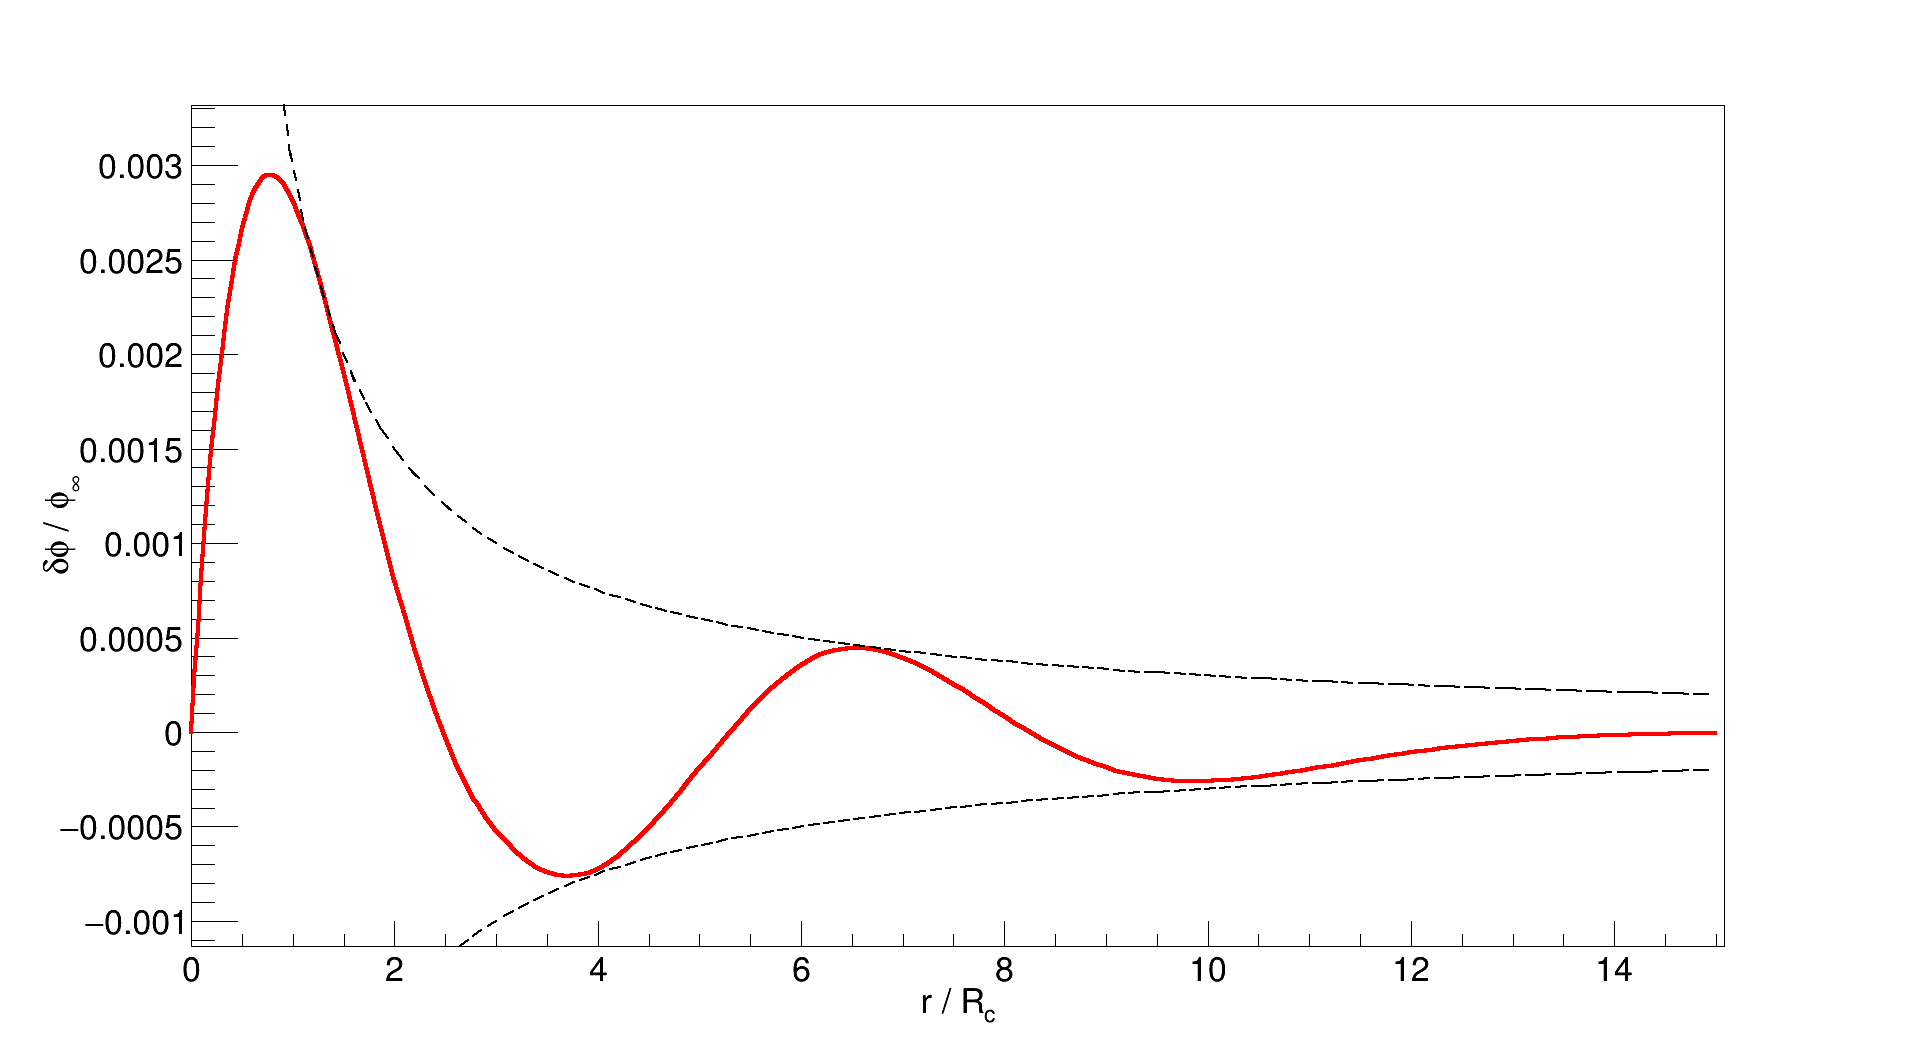
\includegraphics[width=6.5cm]{Images/P_t11.png}

    \centering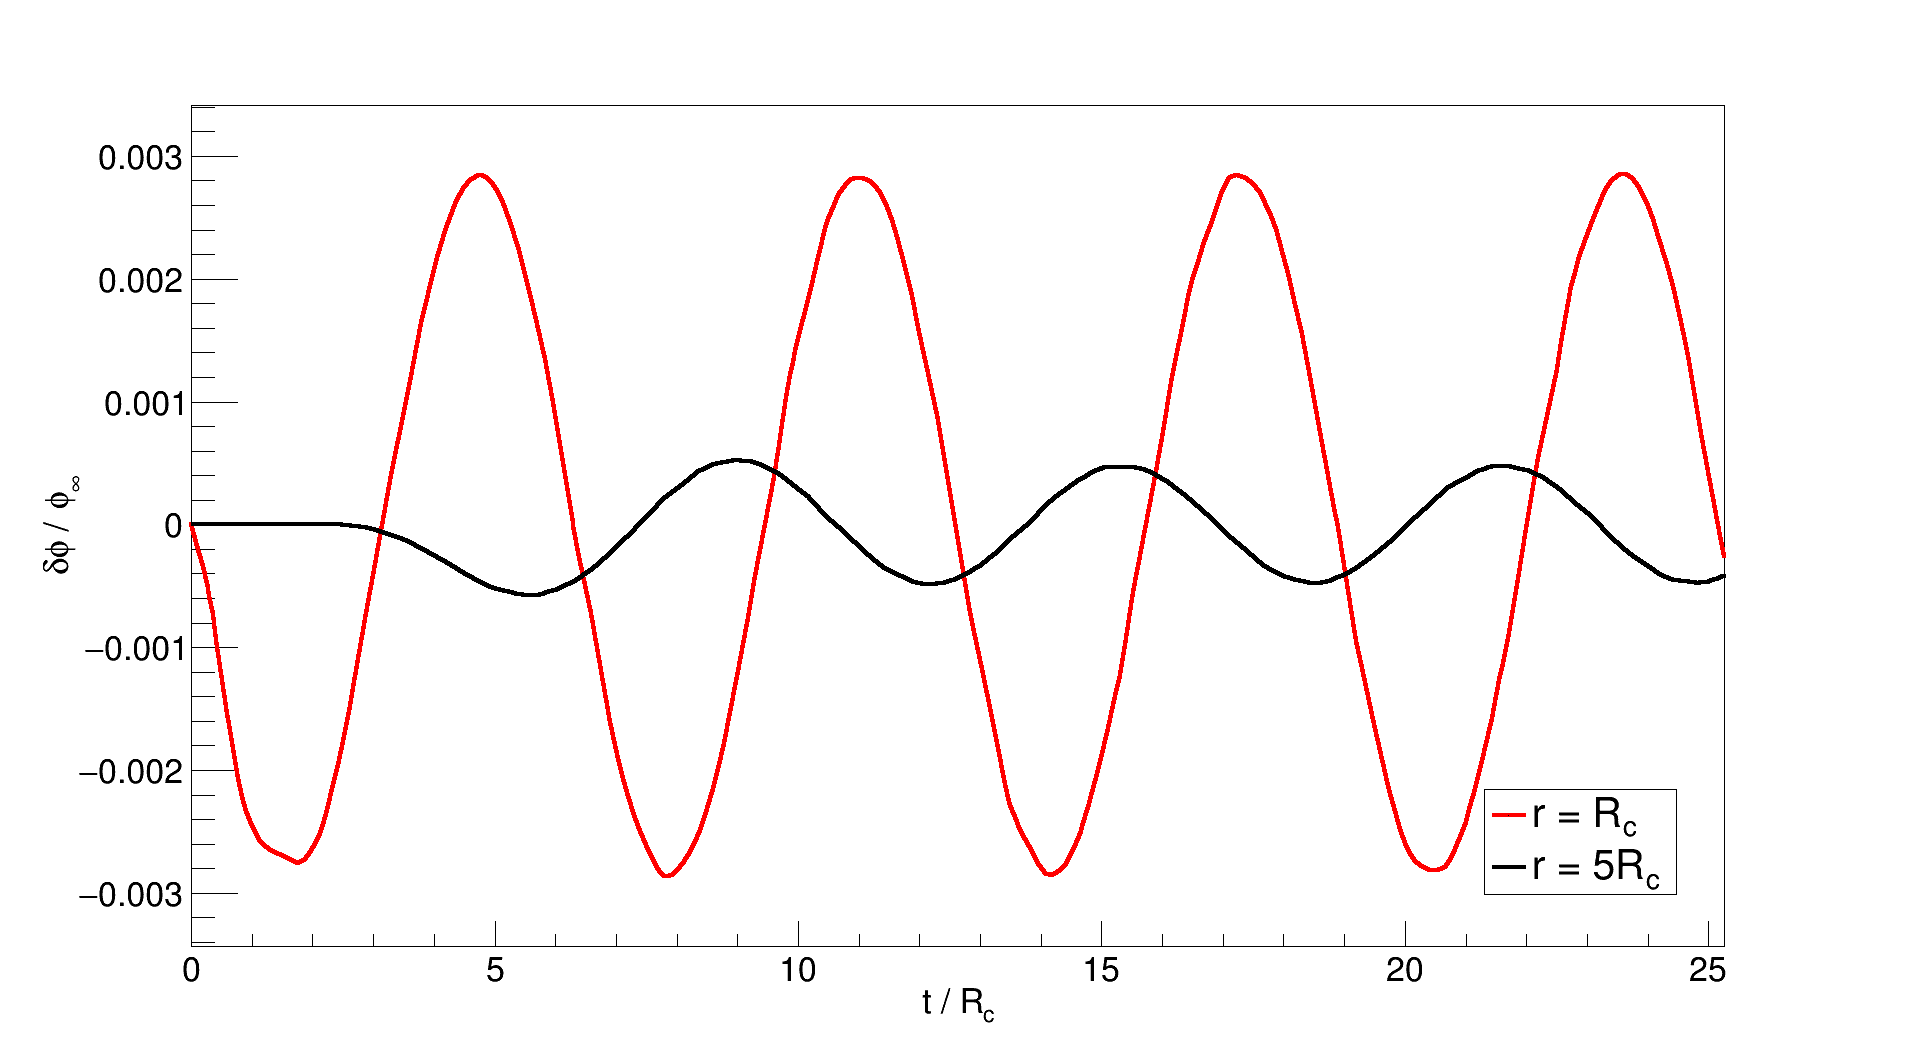
\includegraphics[width=6.5cm]{Images/P_r.png}
\end{column}
\begin{column}{0.35\textwidth}
\vspace{1cm}
\small Perturbations profile at $\tau = 11$ as a function of $x$

\vspace{2.7cm}
\small Perturbations profile at $x = 1$ and $x =5$ as a function of $\tau$

\end{column}
\end{columns}


\end{frame}

\begin{frame}
\frametitle{Scalar energy loss}

\begin{columns}[T]
\begin{column}{0.7\textwidth}
        \begin{equation*}
        \tcbhighmath[boxrule=2pt,arc=1pt,colback=blue!10!white,colframe=blue]{\left.\frac{dE}{dt} = \int_{\partial V}  \Dot{\phi}\partial_i\phi n_i \: dS = 4\pi R^2 \frac{\partial \phi}{\partial t}\frac{\partial\phi}{\partial r}\right\rvert_{r=R}}
    \end{equation*}
\end{column}
\begin{column}{0.3\textwidth}
\vspace{5mm}
    \begin{equation*}
        \small E = \frac{4}{3}\pi R_c^3\rho_c
    \end{equation*} 
\end{column}

\end{columns}
\vspace{1cm}
\begin{columns}[T]
\begin{column}{0.7\textwidth}
    \centering 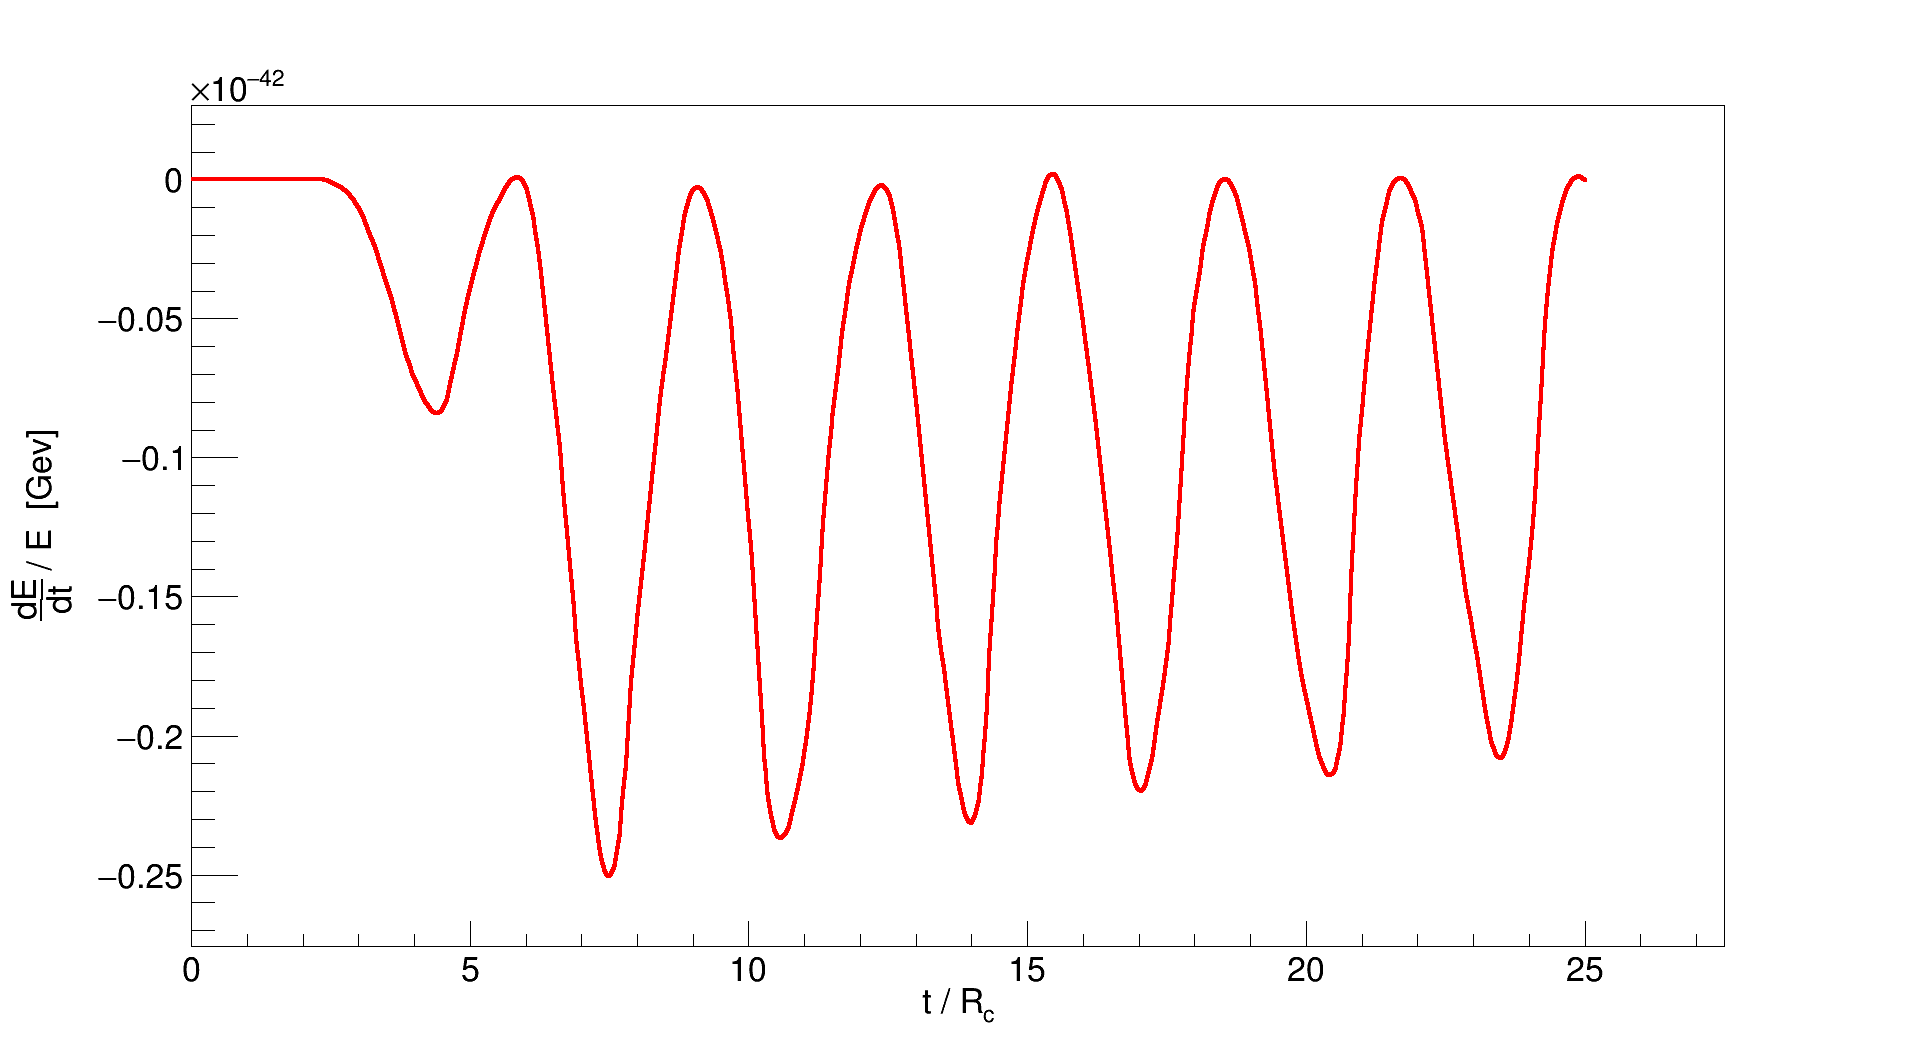
\includegraphics[width=7cm]{Images/Power.png}
    
    \centering \scriptsize Relative power loss $\frac{1}{E}\frac{dE}{dt}$ over time
\end{column}
\begin{column}{0.5\textwidth}
\vspace{2cm}
     \centering\normalsize \tcbhighmath[boxrule=2pt,arc=1pt,colback=white,colframe=red]{$\left\langle \frac{1}{E}\frac{dE}{dt} \right\rangle \approx 10^{-19} s^{-1}$}
\end{column}

\end{columns}
\end{frame}

\begin{frame}{Conclusions}
    \begin{itemize}[<+->]
        \centering  \item Radial pulsations of astrophysical objects source scalar waves
        \item These waves carry energy with them in the form of scalar radiation
        \item Scalar radiation is subdominant when compared to gravitational waves, making them harder to detect
        \item A more realistic result can be obtained by considering GR and using a more accurate model of binary systems
        
    \end{itemize}
    \vspace{5mm}
    \centering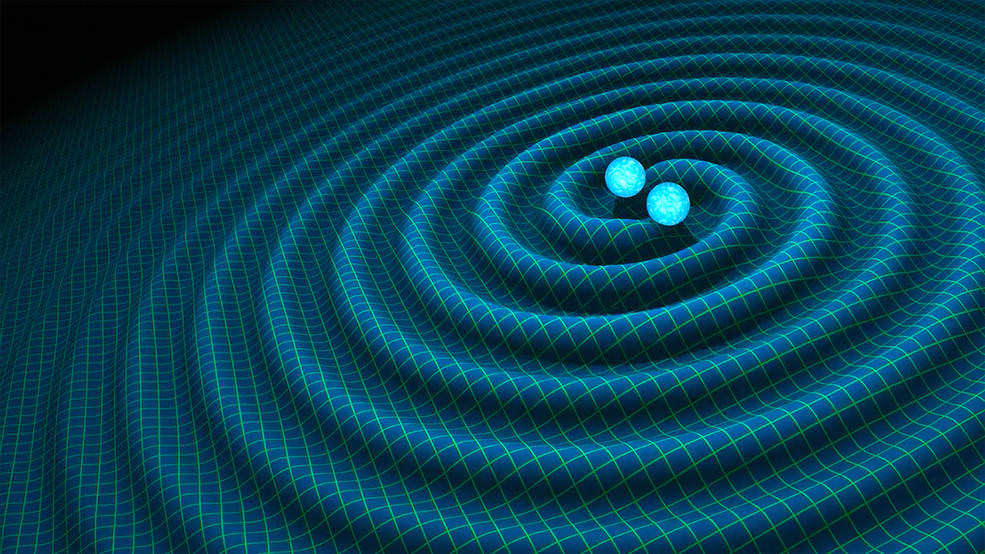
\includegraphics[width=6.5cm]{Images/ns_gw_art.jpg}
\end{frame}

\begin{frame}{Acknowledgements}
    \vspace{3cm}
    \centering \Huge Thank you!
\end{frame}

\end{document}